C++ Lambda表达式,也称为匿名函数、未命名函数、闭包。本节介绍了如何将内核表示为C++ Lambda。本节扩展了第1章中关于C++ Lambda函数的介绍。\par

C++ Lambda表达式非常强大,表示内核时,只需要(并支持)完整C++ Lambda语法的子集即可。\par

\hspace*{\fill} \par %插入空行
图10-2 使用Lambda表达式定义的内核
\begin{lstlisting}[caption={}]
h.parallel_for(size,
	// This is the start of a kernel lambda expression:
	[=](id<1> i) {
		data_acc[i] = data_acc[i] + 1;
	}
	// This is the end of the kernel lambda expression.
);
\end{lstlisting}

\hspace*{\fill} \par %插入空行
\textbf{内核Lambda的构成}

图10-2展示了用Lambda编写的内核———书中目前为止的代码示例都使用这种语法。\par

图10-3中的图显示了可以与内核一起使用的Lambda的更多组件,其中许多都不是必须的。大多数情况下,默认值就足够了,所以内核Lambda看起来更像图10-2中的表达式,而不是图10-3中那样。\par

\hspace*{\fill} \par %插入空行
图10-3 内核Lambda的更多要素,包括可选组件
\begin{center}
	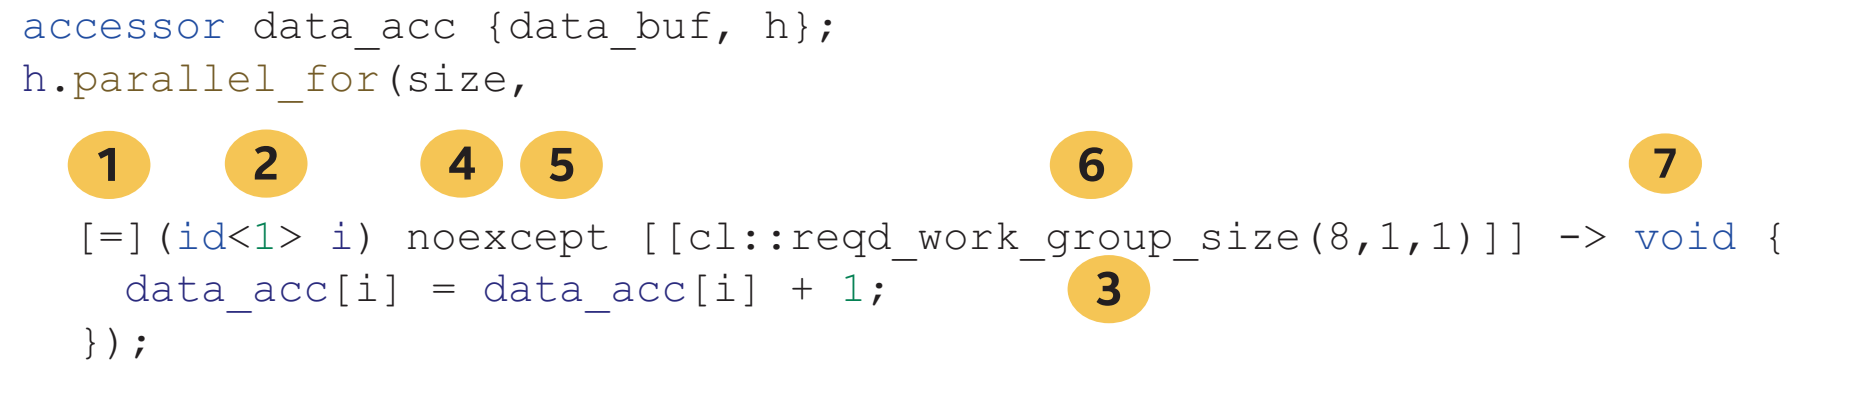
\includegraphics[width=1.0\textwidth]{content/chapter-10/images/2}
\end{center}

\begin{enumerate}
	\item Lambda的第一部分描述捕获。从周围捕获变量使其可以在Lambda表达式中使用,而不用显式地将其作为参数传递给表达式。\\
	C++ Lambda表达式支持通过复制或创建对变量的引用的方式来捕获变量,但对于内核Lambda,变量只能通过复制来捕获。一般的做法是简单地使用默认捕获模式[=],隐式地按值捕获所有变量,不过也可以显式地命名每个捕获的变量。在内核中使用的任何未捕获的变量都会将导致编译时错误。
	\item Lambda的第二部分是传递给表达式的参数,就像传递参数给命名函数一样。\\
	对于内核Lambda,参数取决于调用内核的方式,并且通常标识为并行执行空间中工作项的索引。关于各种并行执行空间,以及如何识别执行空间中工作项的索引的细节信息,请参阅第4章。
	\item Lambda的最后一部分定义了函数体。对于内核Lambda,函数体描述了在并行执行空间中的每个索引处执行的操作。\\
	内核也支持Lambda的其他部分,要么是可选的,要么不常用:
	\item 可能会支持一些说明符(比如mutable),但不建议使用,并且在未来的SYCL版本(在SYCL 2020中已经没有了)或DPC++中可能会删除这种支持。
	\item 如果提供了异常,就必须是noexcept,因为内核不支持异常。
	\item 支持Lambda属性,可以用来控制如何编译内核。例如,reqd\_work\_group\_size属性可用与定义工作组大小。
	\item 可以指定返回类型,但必须返回void,因为内核不支持非void返回类型。
\end{enumerate}

\begin{tcolorbox}[colback=blue!5!white,colframe=blue!75!black, title=Lambda:隐式捕获还是显式捕获?]
一些C++风格指南建议不要使用隐式(或默认)捕获Lambda,因为可能存在悬空指针问题,特别是在表达式跨越作用域边界时。当Lambda用于表示内核时,也会出现同样的问题,因为内核在设备上与主机代码异步执行。\\

因为隐式捕获简单好用,是SYCL内核的常见做法,也是本书中经常使用的一种方法,但最终需要权衡隐式捕获的简洁和显式捕获的清晰。
\end{tcolorbox}

\hspace*{\fill} \par %插入空行
\textbf{命名表示内核的Lambda}

当内核写成Lambda时,某些情况下必须提供另外一个标识:因为表达式是匿名的,有时SYCL需要显式的内核名称模板参数来标识写成表达式的内核。\par

\hspace*{\fill} \par %插入空行
图10-4 命名内核的Lambda
\begin{lstlisting}[caption={}]
// In this example, "class Add" names the kernel lambda:

h.parallel_for<class Add>(size, [=](id<1> i) {
	data_acc[i] = data_acc[i] + 1;
});
\end{lstlisting}

命名内核Lambda是由主机代码编译器确定,再由单独的设备代码编译器编译内核时,确定调用哪个内核的一种方法。命名内核Lambda还可以对已编译的内核进行运行时选择,或通过名称构建内核,如图10-9所示。\par

为了在不需要内核名的情况下支持更简洁的代码,DPC++编译器支持通过-fsyclnamed -lambda编译器选项来省略内核名。使用该选项时,不需要显式的内核名模板参数,如图10-5所示。\par

\hspace*{\fill} \par %插入空行
图10-5 使用未命名的内核Lambda
\begin{lstlisting}[caption={}]
// In many cases the explicit kernel name template parameter
// is not required.
h.parallel_for(size, [=](id<1> i) {
	data_acc[i] = data_acc[i] + 1;
});
\end{lstlisting}

大多数情况下不需要Lambda的内核名称模板参数,所以可以从未命名的Lambda开始,只有在需要内核名称的情况下添加即可。\par

\begin{tcolorbox}[colback=red!5!white,colframe=red!75!black]
不需要内核名称时,首选未命名的内核Lambda。
\end{tcolorbox}



















